\begin{adjustwidth*}{}{-2.25in}
\textbf{{\large Exercises}}
\setlength{\columnsep}{25pt}
\begin{multicols*}{2}
\noindent Terms and Concepts \small
\begin{enumerate}[1)]
\item T/F: Every function has an inverse.
\item In your own words explain what it means for a function to be ``one to one.''
\item If $(1,10)$ lies on the graph of $y=f(x)$, what can be said about the graph of $y=f^{-1}(x)$?
\item If $(1,10)$ lies on the graph of $y=f(x)$ and $\fp(1) = 5$, what can be said about $y=f^{-1}(x)$?
\end{enumerate} 

\noindent {\normalsize Problems} \small

\noindent {\bf In exercises 5--8, verify that the given functions are inverses.}

\begin{enumerate}[1),resume]
\item $\ds f(x) = 2x+6$ and $g(x) = \frac12x-3$
\item $\ds f(x) = x^2+6x+11$, $x\geq 3$ and 

$g(x) = \sqrt{x-2}-3$, $x\geq 2$
\item $\ds f(x) = \frac{3}{x-5}$, $x\neq 5$ and 

$\ds g(x) = \frac{3+5x}{x}$, $x\neq 0$
\item $\ds f(x) = \frac{x+1}{x-1}$, $x\neq 1$ and $g(x) = f(x)$
\end{enumerate}

\noindent {\bf In exercises 9--14, an invertible function $f(x)$ is given along with a point that lies on its graph.  Evaluate $\left( f^{-1} \right)'(x)$ at the indicated value.}

\begin{enumerate}[1),resume]
\item $\ds f(x) = 5x+10$

Point$=(2,20)$ 

Evaluate $\left(f^{-1}\right)'(20)$

\item $\ds f(x) = x^2-2x+4$, $x\geq 1$

Point$=(3,7)$ 

Evaluate $\left(f^{-1}\right)'(7)$

\item $\ds f(x) = \sin 2x$, $-\pi/4\leq x\leq \pi/4$

Point$=(\pi/6,\sqrt{3}/2)$ 

Evaluate $\left(f^{-1}\right)'(\sqrt{3}/2)$

\item $\ds f(x) = x^3-6x^2+15x-2$

Point$=(1,8)$ 

Evaluate $\left(f^{-1}\right)'(8)$

\item $\ds f(x) = \frac{1}{1+x^2}$, $x\geq 0$

Point$=(1,1/2)$ 

Evaluate $\left(f^{-1}\right)'(1/2)$

\item $\ds f(x) = 6e^{3x}$

Point$=(0,6)$ 

Evaluate $\left(f^{-1}\right)'(6)$
\end{enumerate}

\noindent {\bf In exercises 15--28, compute the derivative of the given function.}

\begin{enumerate}[1),resume]
\item $\ds h(t) = \arcsin(2t)$

\item $\ds f(t) = \arcsec(2t)$

\item $\ds g(x) = \arctan(2x)$

\item $\ds f(x) = x \arcsin(x)$

\item $\ds g(t) = \sin(t) \arccos(t)$

\item $\ds f(t) = \ln(t e^t)$

\item $\ds h(x) = \frac{\arcsin(x)}{\arccos(x)}$

\item $\ds g(x) = \arctan(\sqrt{x})$

\item $\ds f(x) = \arcsec(1/x)$

\item $\ds f(x) = \sin(\arcsin(x))$

	\item $f(x) = \ln(2\arctan(x) + 3\arcsin(x) + 5)$
	\item $r(z) = \arctan(\ln(\arcsin(z)))$
	\item $q(t) = \arctan^2(3t) \arcsin^4(7t)$ 
	\item $\ds g(v) =  \ln\left( \frac{\arctan(v)}{\arcsin(v) + v^2} \right)$
\end{enumerate}

\noindent {\bf In exercises 29--34, use logarithmic differentiation to find $\frac{dy}{dx}$, then find the equation of the tangent line at the indicated $x$-value.}

\begin{enumerate}[1),resume]
\item $\ds y=(1+x)^{1/x}$,\quad $x=1$
\item $\ds y=(2x)^{x^2}$,\quad $x=1$
\item $\ds y=\frac{x^{x}}{x+1}$,\quad $x=1$
\item $\ds y=x^{\sin (x)+2}$,\quad $x=\pi/2$
\item $\ds y=\frac{x+1}{x+2}$,\quad $x=1$
\item $\ds y=\frac{(x+1)(x+2)}{(x+3)(x+4)}$,\quad $x=0$
\end{enumerate}

\noindent {\bf In exercises 35--36, find the equation of the tangent line to the graph of the function at the indicated value.}

\begin{enumerate}[1),resume]
\item $\ds f(x) = \arcsin(x)$ at $x = \frac{\sqrt{2}}{2}$
\item $\ds f(x) = \arccos(2x)$ at $x = \frac{\sqrt{3}}{4}$

\item Let $f(x) = \frac{1}{4}x^3 + 4.$
\ba
	\item Sketch a graph of $y = f(x)$ and explain why $f$ is an invertible function.
	\item Let $g$ be the inverse of $f$ and determine a formula for $g$.
	\item Compute $f'(x)$, $g'(x)$, $f'(2)$, and $g'(6)$.  What is the special relationship between $f'(2)$ and $g'(6)$?  Why?
\ea

\end{enumerate}

%------------------------------------------
% END OF EXERCISES ON FIRST PAGE
%------------------------------------------
\end{multicols*}
\end{adjustwidth*}

\clearpage

\begin{adjustwidth*}{}{-2.25in}
\setlength{\columnsep}{25pt}
\begin{multicols*}{2}\small

\begin{enumerate}[1),start=38]

\item Consider the graph of $y = f(x)$ provided below and use it to answer the following questions.
\begin{center}
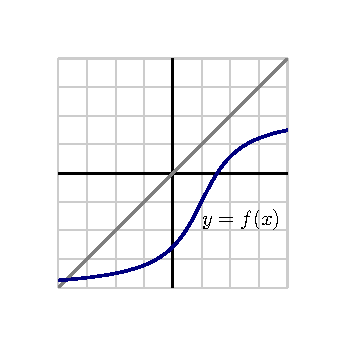
\includegraphics[scale=.75]{figures/2_6_Ez4.eps}
\end{center}
\ba
	\item Use the provided graph to estimate the value of $f'(1)$.
	\item Sketch an approximate graph of $y = f^{-1}(x)$.  Label at least three distinct points on the graph that correspond to three points on the graph of $f$.
	\item Based on your work in (a), what is the value of $(f^{-1})'(-1)$?  Why?
\ea

\item Let $h(x) = x + \sin(x)$.
\ba
	\item Sketch a graph of $y = h(x)$ and explain why $h$ must be invertible.
	\item Explain why it does not appear to be algebraically possible to determine a formula for $h^{-1}$.
	\item Observe that the point $(\frac{\pi}{2}, \frac{\pi}{2} + 1)$ lies on the graph of $y = h(x)$.  Determine the value of $(h^{-1})'(\frac{\pi}{2} + 1)$.
\ea
\end{enumerate}

%---------------------------------------------
% END OF EXERCISES ON SECOND PAGE
%---------------------------------------------
\end{multicols*}
\end{adjustwidth*}

\afterexercises